\section{Processing the Final Thesis}

\subsection{Writing Academic Text}

When writing final theses, it is appropriate to follow the principles of academic writing:

\begin{itemize}
	\item Academic text uses stylistic means that avoid repeated use of the word “I”. One option is the use of the authorial or modest plural, which is common in definitional processes (We denote the object as,…). Impersonal expression can also be achieved by using passive constructions (The third chapter is supplemented…, were described,…).
	\item In academic text, certain types of expressions appear, referring to:
	\begin{itemize}
		\item location: as stated above / below, in the following chapter,…
		\item time: so far we have discussed…, before we proceed to the explanation…
		\item process: if we return to the function…, we concluded…
	\end{itemize}
	\item The author’s own ideas must be separated from ideas taken from other sources, which must be cited.
\end{itemize}

\subsubsection{Punctuation Marks}

\paragraph{Hyphen and Dash}

A hyphen is written using the division mark without spaces. The hyphen connects:

\begin{itemize}
	\item two words to express the relationship of originally separate words,
	\item individual parts of compound words expressed by numbers and letters,
	\item an initial abbreviation and a suffix.
\end{itemize}

Examples: Rázusová-Martáková, more-or-less, step-by-step, material-technical, Slovak-Czech, white-blue, 3-part, 10-percent, 2-room, in TANAP.

A dash is written with spaces on both sides. If a dash appears at the end of a line, it is not repeated at the beginning of the next line. A dash is most often used:

\begin{itemize}
	\item when separating a parenthetical clause in a sentence,
	\item after an expression or statement that is not further explained,
	\item when indicating a range or an equivalence relationship between two or more items (time and location ranges, directions, stations on a route, sports matches, negotiation partners, co-authors or co-organizers, etc.).
\end{itemize}

Examples: At the meeting they discussed – among other things – the archiving of documents. The dismissal was justified – a serious violation of work regulations occurred. 11–14 July 2010, 1998–2002, pages 3–7, § 13–§ 15, Bratislava – Žilina – Poprad-Tatry – Košice, Kováč – Schuster, Janošová – Kuláková...

\paragraph{Period, Exclamation Mark, Question Mark, Comma, Semicolon, Colon, Parentheses}

A period, exclamation mark, question mark, comma, semicolon, and colon are written directly after the corresponding word without a space. If more punctuation marks follow a word or appear at the end of a sentence, the space is placed only after the last one. If a sentence ends with an abbreviation, the period after the abbreviation serves as the sentence-ending period. If parentheses are used within a sentence, the period is written after the closing parenthesis. If the text inside parentheses is a complete sentence, even a one-word or elliptical one, the period is written before the closing parenthesis.

\subsection{Abbreviations, Technical Terms, and Source Citations}

Introduce English technical terms at their first occurrence in the text, and if possible, include the abbreviation in parentheses and use only the abbreviation later. Example: Access point (AP). Do not forget to include a list of all abbreviations used in the thesis at the beginning.

If a commonly used Slovak translation of an English term exists, use the Slovak term in the thesis, for example smerovač (router), prepínač (switch).

A period is written after established textual abbreviations, followed by a space. If more punctuation marks follow the abbreviation, the space is placed only after the last one.

Examples: č. = number, str. = page, Z. z. = Collection of Laws, ods. = paragraph

\subsection{Figures}

Figure~\ref{fig:testpicture} shows an communication between a client and a RADIUS server.

\begin{figure}[tbph]
	\centering
	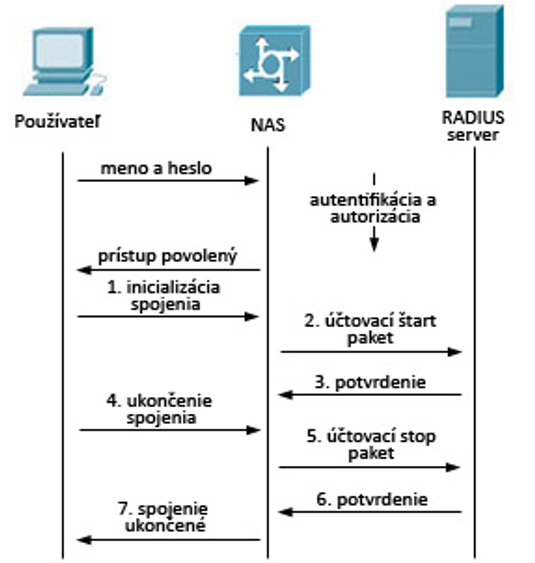
\includegraphics[width=0.6\linewidth]{pictures/test_picture}
	\caption{Test image}
	\label{fig:testpicture}
	\smallskip
	{\footnotesize Source: own processing}
\end{figure}

\subsection{Tables}

Table~\ref{tab:si_units} lists the basic units in electronics.

\begin{table}[htbp] 
	\centering 
	\caption{Basic units in electronics}
	\label{tab:si_units}
	
	% X - collumn content alligned to left
	% c - collumn content alligned to center
	\begin{tabularx}{0.8\linewidth}{X X c}
		\toprule
		\textbf{Quantity} & \textbf{Unit} & \textbf{Symbol} \\
		\midrule
		
		% --- Block title 1 ---
		\multicolumn{3}{c}{\textbf{Technical Block 1}} \\
		\addlinespace[2pt]
		
		% --- Block 1 ---
		\glsentrydesc{sym:U} & \glsentryuserii{sym:U} [\glsentryuseri{sym:U}] & \gls{sym:U} \\
		\glsentrydesc{sym:R} & \glsentryuserii{sym:R} [\glsentryuseri{sym:R}] & \gls{sym:R} \\
		\glsentrydesc{sym:I} & \glsentryuserii{sym:I} [\glsentryuseri{sym:I}] & \gls{sym:I} \\
		
		\midrule % --- Block separation ---
		
		% --- Block title 2 ---
		\multicolumn{3}{c}{\textbf{Technical Block 2}} \\
		\addlinespace[2pt]
		
		% --- Block 2 ---
		\glsentrydesc{sym:U} & \glsentryuserii{sym:U} [\glsentryuseri{sym:U}] & \gls{sym:U} \\
		\glsentrydesc{sym:R} & \glsentryuserii{sym:R} [\glsentryuseri{sym:R}] & \gls{sym:R} \\
		\glsentrydesc{sym:I} & \glsentryuserii{sym:I} [\glsentryuseri{sym:I}] & \gls{sym:I} \\
		
		\bottomrule
	\end{tabularx}

	
	
	\smallskip
	\begin{center}
		{\footnotesize Source: own processing}
	\end{center}
\end{table}

\subsection{Equations}

Ohm’s law expresses the relationship between electric voltage, electric current, and electric resistance:

\begin{equation} 
	\gls{sym:U} = \gls{sym:R} \cdot \gls{sym:I} 
	\label{eq:ohm} 
\end{equation} 

where

\begin{description}
	\item[\gls{sym:U}] \glsentrydesc{sym:U} [\glsentryuseri{sym:U}],
	\item[\gls{sym:R}] \glsentrydesc{sym:R} [\glsentryuseri{sym:R}],
	\item[\gls{sym:I}] \glsentrydesc{sym:I} [\glsentryuseri{sym:I}].
\end{description}

As stated in equation~(\ref{eq:ohm}), electric voltage is directly proportional to electric current.

\subsection{Abbreviations, Citation of Used Literature and units}

\gls{bms} are essential for electric vehicles. The \gls{cpu} processes instructions in assembly language \cite{nuclear_fission_uranium_235, JAYABAL2024103121}.

When working with units, the \texttt{siunitx} package is used, which generates units as follows: \SI{4.00}{\celsius}, \SI{26.4}{\centi\metre}, \SI{0.322}{\milli\watt\per\cubic\centi\metre}, \SI{1}{\percent}, \SI{}{\celsius}.
